\documentclass[11pt,compress,t,notes=noshow, xcolor=table]{beamer}

\documentclass[11pt,compress,t,notes=noshow, xcolor=table]{beamer}
\usepackage[]{graphicx}\usepackage[]{color}
% maxwidth is the original width if it is less than linewidth
% otherwise use linewidth (to make sure the graphics do not exceed the margin)
\makeatletter
\def\maxwidth{ %
  \ifdim\Gin@nat@width>\linewidth
    \linewidth
  \else
    \Gin@nat@width
  \fi
}
\makeatother

\definecolor{fgcolor}{rgb}{0.345, 0.345, 0.345}
\newcommand{\hlnum}[1]{\textcolor[rgb]{0.686,0.059,0.569}{#1}}%
\newcommand{\hlstr}[1]{\textcolor[rgb]{0.192,0.494,0.8}{#1}}%
\newcommand{\hlcom}[1]{\textcolor[rgb]{0.678,0.584,0.686}{\textit{#1}}}%
\newcommand{\hlopt}[1]{\textcolor[rgb]{0,0,0}{#1}}%
\newcommand{\hlstd}[1]{\textcolor[rgb]{0.345,0.345,0.345}{#1}}%
\newcommand{\hlkwa}[1]{\textcolor[rgb]{0.161,0.373,0.58}{\textbf{#1}}}%
\newcommand{\hlkwb}[1]{\textcolor[rgb]{0.69,0.353,0.396}{#1}}%
\newcommand{\hlkwc}[1]{\textcolor[rgb]{0.333,0.667,0.333}{#1}}%
\newcommand{\hlkwd}[1]{\textcolor[rgb]{0.737,0.353,0.396}{\textbf{#1}}}%
\let\hlipl\hlkwb

\usepackage{framed}
\makeatletter
\newenvironment{kframe}{%
 \def\at@end@of@kframe{}%
 \ifinner\ifhmode%
  \def\at@end@of@kframe{\end{minipage}}%
  \begin{minipage}{\columnwidth}%
 \fi\fi%
 \def\FrameCommand##1{\hskip\@totalleftmargin \hskip-\fboxsep
 \colorbox{shadecolor}{##1}\hskip-\fboxsep
     % There is no \\@totalrightmargin, so:
     \hskip-\linewidth \hskip-\@totalleftmargin \hskip\columnwidth}%
 \MakeFramed {\advance\hsize-\width
   \@totalleftmargin\z@ \linewidth\hsize
   \@setminipage}}%
 {\par\unskip\endMakeFramed%
 \at@end@of@kframe}
\makeatother

\definecolor{shadecolor}{rgb}{.97, .97, .97}
\definecolor{messagecolor}{rgb}{0, 0, 0}
\definecolor{warningcolor}{rgb}{1, 0, 1}
\definecolor{errorcolor}{rgb}{1, 0, 0}
\newenvironment{knitrout}{}{} % an empty environment to be redefined in TeX

\usepackage{alltt}
\newcommand{\SweaveOpts}[1]{}  % do not interfere with LaTeX
\newcommand{\SweaveInput}[1]{} % because they are not real TeX commands
\newcommand{\Sexpr}[1]{}       % will only be parsed by R
\newcommand{\xmark}{\ding{55}}%


\usepackage[english]{babel}
\usepackage[utf8]{inputenc}

\usepackage{dsfont}
\usepackage{verbatim}
\usepackage{amsmath}
\usepackage{amsfonts}
\usepackage{amssymb}
\usepackage{bm}
\usepackage{csquotes}
\usepackage{multirow}
\usepackage{longtable}
\usepackage{booktabs}
\usepackage{enumerate}
\usepackage[absolute,overlay]{textpos}
\usepackage{psfrag}
\usepackage{algorithm}
\usepackage{algpseudocode}
\usepackage{eqnarray}
\usepackage{arydshln}
\usepackage{tabularx}
\usepackage{placeins}
\usepackage{tikz}
\usepackage{setspace}
\usepackage{colortbl}
\usepackage{mathtools}
\usepackage{wrapfig}
\usepackage{bm}
\usepackage{amsmath}
\usepackage{pifont}

\usetikzlibrary{shapes,arrows,automata,positioning,calc,chains,trees, shadows}
\tikzset{
  %Define standard arrow tip
  >=stealth',
  %Define style for boxes
  punkt/.style={
    rectangle,
    rounded corners,
    draw=black, very thick,
    text width=6.5em,
    minimum height=2em,
    text centered},
  % Define arrow style
  pil/.style={
    ->,
    thick,
    shorten <=2pt,
    shorten >=2pt,}
}

\usepackage{subfig}

% Defines macros and environments
\usepackage{../../style/lmu-lecture}


\let\code=\texttt
\let\proglang=\textsf

\setkeys{Gin}{width=0.9\textwidth}

\setbeamertemplate{frametitle}{\expandafter\uppercase\expandafter\insertframetitle}

\usepackage{bbm}
% basic latex stuff
\newcommand{\pkg}[1]{{\fontseries{b}\selectfont #1}} %fontstyle for R packages
\newcommand{\lz}{\vspace{0.5cm}} %vertical space
\newcommand{\dlz}{\vspace{1cm}} %double vertical space
\newcommand{\oneliner}[1] % Oneliner for important statements
{\begin{block}{}\begin{center}\begin{Large}#1\end{Large}\end{center}\end{block}}


%new environments
\newenvironment{vbframe}  %frame with breaks and verbatim
{
 \begin{frame}[containsverbatim,allowframebreaks]
}
{
\end{frame}
}

\newenvironment{vframe}  %frame with verbatim without breaks (to avoid numbering one slided frames)
{
 \begin{frame}[containsverbatim]
}
{
\end{frame}
}

\newenvironment{blocki}[1]   % itemize block
{
 \begin{block}{#1}\begin{itemize}
}
{
\end{itemize}\end{block}
}

\newenvironment{fragileframe}[2]{  %fragile frame with framebreaks
\begin{frame}[allowframebreaks, fragile, environment = fragileframe]
\frametitle{#1}
#2}
{\end{frame}}


\newcommand{\myframe}[2]{  %short for frame with framebreaks
\begin{frame}[allowframebreaks]
\frametitle{#1}
#2
\end{frame}}

\newcommand{\remark}[1]{
  \textbf{Remark:} #1
}


\newenvironment{deleteframe}
{
\begingroup
\usebackgroundtemplate{
\includegraphics[width=\paperwidth,height=\paperheight]{../style/color/red.png}}
 \begin{frame}
}
{
\end{frame}
\endgroup
}
\newenvironment{simplifyframe}
{
\begingroup
\usebackgroundtemplate{
\includegraphics[width=\paperwidth,height=\paperheight]{../style/color/yellow.png}}
 \begin{frame}
}
{
\end{frame}
\endgroup
}\newenvironment{draftframe}
{
\begingroup
\usebackgroundtemplate{
\includegraphics[width=\paperwidth,height=\paperheight]{../style/color/green.jpg}}
 \begin{frame}
}
{
\end{frame}
\endgroup
}
% https://tex.stackexchange.com/a/261480: textcolor that works in mathmode
\makeatletter
\renewcommand*{\@textcolor}[3]{%
  \protect\leavevmode
  \begingroup
    \color#1{#2}#3%
  \endgroup
}
\makeatother





% math spaces
\ifdefined\N                                                                
\renewcommand{\N}{\mathds{N}} % N, naturals
\else \newcommand{\N}{\mathds{N}} \fi 
\newcommand{\Z}{\mathds{Z}} % Z, integers
\newcommand{\Q}{\mathds{Q}} % Q, rationals
\newcommand{\R}{\mathds{R}} % R, reals
\ifdefined\C 
  \renewcommand{\C}{\mathds{C}} % C, complex
\else \newcommand{\C}{\mathds{C}} \fi
\newcommand{\continuous}{\mathcal{C}} % C, space of continuous functions
\newcommand{\M}{\mathcal{M}} % machine numbers
\newcommand{\epsm}{\epsilon_m} % maximum error

% counting / finite sets
\newcommand{\setzo}{\{0, 1\}} % set 0, 1
\newcommand{\setmp}{\{-1, +1\}} % set -1, 1
\newcommand{\unitint}{[0, 1]} % unit interval

% basic math stuff
\newcommand{\xt}{\tilde x} % x tilde
\newcommand{\argmax}{\operatorname{arg\,max}} % argmax
\newcommand{\argmin}{\operatorname{arg\,min}} % argmin
\newcommand{\argminlim}{\mathop{\mathrm{arg\,min}}\limits} % argmax with limits
\newcommand{\argmaxlim}{\mathop{\mathrm{arg\,max}}\limits} % argmin with limits  
\newcommand{\sign}{\operatorname{sign}} % sign, signum
\newcommand{\I}{\mathbb{I}} % I, indicator
\newcommand{\order}{\mathcal{O}} % O, order
\newcommand{\pd}[2]{\frac{\partial{#1}}{\partial #2}} % partial derivative
\newcommand{\floorlr}[1]{\left\lfloor #1 \right\rfloor} % floor
\newcommand{\ceillr}[1]{\left\lceil #1 \right\rceil} % ceiling

% sums and products
\newcommand{\sumin}{\sum\limits_{i=1}^n} % summation from i=1 to n
\newcommand{\sumim}{\sum\limits_{i=1}^m} % summation from i=1 to m
\newcommand{\sumjn}{\sum\limits_{j=1}^n} % summation from j=1 to p
\newcommand{\sumjp}{\sum\limits_{j=1}^p} % summation from j=1 to p
\newcommand{\sumik}{\sum\limits_{i=1}^k} % summation from i=1 to k
\newcommand{\sumkg}{\sum\limits_{k=1}^g} % summation from k=1 to g
\newcommand{\sumjg}{\sum\limits_{j=1}^g} % summation from j=1 to g
\newcommand{\meanin}{\frac{1}{n} \sum\limits_{i=1}^n} % mean from i=1 to n
\newcommand{\meanim}{\frac{1}{m} \sum\limits_{i=1}^m} % mean from i=1 to n
\newcommand{\meankg}{\frac{1}{g} \sum\limits_{k=1}^g} % mean from k=1 to g
\newcommand{\prodin}{\prod\limits_{i=1}^n} % product from i=1 to n
\newcommand{\prodkg}{\prod\limits_{k=1}^g} % product from k=1 to g
\newcommand{\prodjp}{\prod\limits_{j=1}^p} % product from j=1 to p

% linear algebra
\newcommand{\one}{\boldsymbol{1}} % 1, unitvector
\newcommand{\zero}{\mathbf{0}} % 0-vector
\newcommand{\id}{\boldsymbol{I}} % I, identity
\newcommand{\diag}{\operatorname{diag}} % diag, diagonal
\newcommand{\trace}{\operatorname{tr}} % tr, trace
\newcommand{\spn}{\operatorname{span}} % span
\newcommand{\scp}[2]{\left\langle #1, #2 \right\rangle} % <.,.>, scalarproduct
\newcommand{\mat}[1]{\begin{pmatrix} #1 \end{pmatrix}} % short pmatrix command
\newcommand{\Amat}{\mathbf{A}} % matrix A
\newcommand{\Deltab}{\mathbf{\Delta}} % error term for vectors

% basic probability + stats
\renewcommand{\P}{\mathds{P}} % P, probability
\newcommand{\E}{\mathds{E}} % E, expectation
\newcommand{\var}{\mathsf{Var}} % Var, variance
\newcommand{\cov}{\mathsf{Cov}} % Cov, covariance
\newcommand{\corr}{\mathsf{Corr}} % Corr, correlation
\newcommand{\normal}{\mathcal{N}} % N of the normal distribution
\newcommand{\iid}{\overset{i.i.d}{\sim}} % dist with i.i.d superscript
\newcommand{\distas}[1]{\overset{#1}{\sim}} % ... is distributed as ...

% machine learning
\newcommand{\Xspace}{\mathcal{X}} % X, input space
\newcommand{\Yspace}{\mathcal{Y}} % Y, output space
\newcommand{\nset}{\{1, \ldots, n\}} % set from 1 to n
\newcommand{\pset}{\{1, \ldots, p\}} % set from 1 to p
\newcommand{\gset}{\{1, \ldots, g\}} % set from 1 to g
\newcommand{\Pxy}{\mathbb{P}_{xy}} % P_xy
\newcommand{\Exy}{\mathbb{E}_{xy}} % E_xy: Expectation over random variables xy
\newcommand{\xv}{\mathbf{x}} % vector x (bold)
\newcommand{\xtil}{\tilde{\mathbf{x}}} % vector x-tilde (bold)
\newcommand{\yv}{\mathbf{y}} % vector y (bold)
\newcommand{\xy}{(\xv, y)} % observation (x, y)
\newcommand{\xvec}{\left(x_1, \ldots, x_p\right)^\top} % (x1, ..., xp) 
\newcommand{\Xmat}{\mathbf{X}} % Design matrix
\newcommand{\allDatasets}{\mathds{D}} % The set of all datasets
\newcommand{\allDatasetsn}{\mathds{D}_n}  % The set of all datasets of size n 
\newcommand{\D}{\mathcal{D}} % D, data
\newcommand{\Dn}{\D_n} % D_n, data of size n
\newcommand{\Dtrain}{\mathcal{D}_{\text{train}}} % D_train, training set
\newcommand{\Dtest}{\mathcal{D}_{\text{test}}} % D_test, test set
\newcommand{\xyi}[1][i]{\left(\xv^{(#1)}, y^{(#1)}\right)} % (x^i, y^i), i-th observation
\newcommand{\Dset}{\left( \xyi[1], \ldots, \xyi[n]\right)} % {(x1,y1)), ..., (xn,yn)}, data
\newcommand{\defAllDatasetsn}{(\Xspace \times \Yspace)^n} % Def. of the set of all datasets of size n 
\newcommand{\defAllDatasets}{\bigcup_{n \in \N}(\Xspace \times \Yspace)^n} % Def. of the set of all datasets 
\newcommand{\xdat}{\left\{ \xv^{(1)}, \ldots, \xv^{(n)}\right\}} % {x1, ..., xn}, input data
\newcommand{\ydat}{\left\{ \yv^{(1)}, \ldots, \yv^{(n)}\right\}} % {y1, ..., yn}, input data
\newcommand{\yvec}{\left(y^{(1)}, \hdots, y^{(n)}\right)^\top} % (y1, ..., yn), vector of outcomes
\renewcommand{\xi}[1][i]{\xv^{(#1)}} % x^i, i-th observed value of x
\newcommand{\yi}[1][i]{y^{(#1)}} % y^i, i-th observed value of y 
\newcommand{\xivec}{\left(x^{(i)}_1, \ldots, x^{(i)}_p\right)^\top} % (x1^i, ..., xp^i), i-th observation vector
\newcommand{\xj}{\xv_j} % x_j, j-th feature
\newcommand{\xjvec}{\left(x^{(1)}_j, \ldots, x^{(n)}_j\right)^\top} % (x^1_j, ..., x^n_j), j-th feature vector
\newcommand{\phiv}{\mathbf{\phi}} % Basis transformation function phi
\newcommand{\phixi}{\mathbf{\phi}^{(i)}} % Basis transformation of xi: phi^i := phi(xi)

%%%%%% ml - models general
\newcommand{\lamv}{\bm{\lambda}} % lambda vector, hyperconfiguration vector
\newcommand{\Lam}{\bm{\Lambda}}	 % Lambda, space of all hpos
% Inducer / Inducing algorithm
\newcommand{\preimageInducer}{\left(\defAllDatasets\right)\times\Lam} % Set of all datasets times the hyperparameter space
\newcommand{\preimageInducerShort}{\allDatasets\times\Lam} % Set of all datasets times the hyperparameter space
% Inducer / Inducing algorithm
\newcommand{\ind}{\mathcal{I}} % Inducer, inducing algorithm, learning algorithm 

% continuous prediction function f
\newcommand{\ftrue}{f_{\text{true}}}  % True underlying function (if a statistical model is assumed)
\newcommand{\ftruex}{\ftrue(\xv)} % True underlying function (if a statistical model is assumed)
\newcommand{\fx}{f(\xv)} % f(x), continuous prediction function
\newcommand{\fdomains}{f: \Xspace \rightarrow \R^g} % f with domain and co-domain
\newcommand{\Hspace}{\mathcal{H}} % hypothesis space where f is from
\newcommand{\fbayes}{f^{\ast}} % Bayes-optimal model
\newcommand{\fxbayes}{f^{\ast}(\xv)} % Bayes-optimal model
\newcommand{\fkx}[1][k]{f_{#1}(\xv)} % f_j(x), discriminant component function
\newcommand{\fh}{\hat{f}} % f hat, estimated prediction function
\newcommand{\fxh}{\fh(\xv)} % fhat(x)
\newcommand{\fxt}{f(\xv ~|~ \thetab)} % f(x | theta)
\newcommand{\fxi}{f\left(\xv^{(i)}\right)} % f(x^(i))
\newcommand{\fxih}{\hat{f}\left(\xv^{(i)}\right)} % f(x^(i))
\newcommand{\fxit}{f\left(\xv^{(i)} ~|~ \thetab\right)} % f(x^(i) | theta)
\newcommand{\fhD}{\fh_{\D}} % fhat_D, estimate of f based on D
\newcommand{\fhDtrain}{\fh_{\Dtrain}} % fhat_Dtrain, estimate of f based on D
\newcommand{\fhDnlam}{\fh_{\Dn, \lamv}} %model learned on Dn with hp lambda
\newcommand{\fhDlam}{\fh_{\D, \lamv}} %model learned on D with hp lambda
\newcommand{\fhDnlams}{\fh_{\Dn, \lamv^\ast}} %model learned on Dn with optimal hp lambda 
\newcommand{\fhDlams}{\fh_{\D, \lamv^\ast}} %model learned on D with optimal hp lambda 

% discrete prediction function h
\newcommand{\hx}{h(\xv)} % h(x), discrete prediction function
\newcommand{\hh}{\hat{h}} % h hat
\newcommand{\hxh}{\hat{h}(\xv)} % hhat(x)
\newcommand{\hxt}{h(\xv | \thetab)} % h(x | theta)
\newcommand{\hxi}{h\left(\xi\right)} % h(x^(i))
\newcommand{\hxit}{h\left(\xi ~|~ \thetab\right)} % h(x^(i) | theta)
\newcommand{\hbayes}{h^{\ast}} % Bayes-optimal classification model
\newcommand{\hxbayes}{h^{\ast}(\xv)} % Bayes-optimal classification model

% yhat
\newcommand{\yh}{\hat{y}} % yhat for prediction of target
\newcommand{\yih}{\hat{y}^{(i)}} % yhat^(i) for prediction of ith targiet
\newcommand{\resi}{\yi- \yih}

% theta
\newcommand{\thetah}{\hat{\theta}} % theta hat
\newcommand{\thetab}{\bm{\theta}} % theta vector
\newcommand{\thetabh}{\bm{\hat\theta}} % theta vector hat
\newcommand{\thetat}[1][t]{\thetab^{[#1]}} % theta^[t] in optimization
\newcommand{\thetatn}[1][t]{\thetab^{[#1 +1]}} % theta^[t+1] in optimization
\newcommand{\thetahDnlam}{\thetabh_{\Dn, \lamv}} %theta learned on Dn with hp lambda
\newcommand{\thetahDlam}{\thetabh_{\D, \lamv}} %theta learned on D with hp lambda
\newcommand{\mint}{\min_{\thetab \in \Theta}} % min problem theta
\newcommand{\argmint}{\argmin_{\thetab \in \Theta}} % argmin theta

% densities + probabilities
% pdf of x 
\newcommand{\pdf}{p} % p
\newcommand{\pdfx}{p(\xv)} % p(x)
\newcommand{\pixt}{\pi(\xv~|~ \thetab)} % pi(x|theta), pdf of x given theta
\newcommand{\pixit}[1][i]{\pi\left(\xi[#1] ~|~ \thetab\right)} % pi(x^i|theta), pdf of x given theta
\newcommand{\pixii}[1][i]{\pi\left(\xi[#1]\right)} % pi(x^i), pdf of i-th x 

% pdf of (x, y)
\newcommand{\pdfxy}{p(\xv,y)} % p(x, y)
\newcommand{\pdfxyt}{p(\xv, y ~|~ \thetab)} % p(x, y | theta)
\newcommand{\pdfxyit}{p\left(\xi, \yi ~|~ \thetab\right)} % p(x^(i), y^(i) | theta)

% pdf of x given y
\newcommand{\pdfxyk}[1][k]{p(\xv | y= #1)} % p(x | y = k)
\newcommand{\lpdfxyk}[1][k]{\log p(\xv | y= #1)} % log p(x | y = k)
\newcommand{\pdfxiyk}[1][k]{p\left(\xi | y= #1 \right)} % p(x^i | y = k)

% prior probabilities
\newcommand{\pik}[1][k]{\pi_{#1}} % pi_k, prior
\newcommand{\lpik}[1][k]{\log \pi_{#1}} % log pi_k, log of the prior
\newcommand{\pit}{\pi(\thetab)} % Prior probability of parameter theta

% posterior probabilities
\newcommand{\post}{\P(y = 1 ~|~ \xv)} % P(y = 1 | x), post. prob for y=1
\newcommand{\postk}[1][k]{\P(y = #1 ~|~ \xv)} % P(y = k | y), post. prob for y=k
\newcommand{\pidomains}{\pi: \Xspace \rightarrow \unitint} % pi with domain and co-domain
\newcommand{\pibayes}{\pi^{\ast}} % Bayes-optimal classification model
\newcommand{\pixbayes}{\pi^{\ast}(\xv)} % Bayes-optimal classification model
\newcommand{\pix}{\pi(\xv)} % pi(x), P(y = 1 | x)
\newcommand{\piv}{\bm{\pi}} % pi, bold, as vector
\newcommand{\pikx}[1][k]{\pi_{#1}(\xv)} % pi_k(x), P(y = k | x)
\newcommand{\pikxt}[1][k]{\pi_{#1}(\xv ~|~ \thetab)} % pi_k(x | theta), P(y = k | x, theta)
\newcommand{\pixh}{\hat \pi(\xv)} % pi(x) hat, P(y = 1 | x) hat
\newcommand{\pikxh}[1][k]{\hat \pi_{#1}(\xv)} % pi_k(x) hat, P(y = k | x) hat
\newcommand{\pixih}{\hat \pi(\xi)} % pi(x^(i)) with hat
\newcommand{\pikxih}[1][k]{\hat \pi_{#1}(\xi)} % pi_k(x^(i)) with hat
\newcommand{\pdfygxt}{p(y ~|~\xv, \thetab)} % p(y | x, theta)
\newcommand{\pdfyigxit}{p\left(\yi ~|~\xi, \thetab\right)} % p(y^i |x^i, theta)
\newcommand{\lpdfygxt}{\log \pdfygxt } % log p(y | x, theta)
\newcommand{\lpdfyigxit}{\log \pdfyigxit} % log p(y^i |x^i, theta)

% probababilistic
\newcommand{\bayesrulek}[1][k]{\frac{\P(\xv | y= #1) \P(y= #1)}{\P(\xv)}} % Bayes rule
\newcommand{\muk}{\bm{\mu_k}} % mean vector of class-k Gaussian (discr analysis) 

% residual and margin
\newcommand{\eps}{\epsilon} % residual, stochastic
\newcommand{\epsi}{\epsilon^{(i)}} % epsilon^i, residual, stochastic
\newcommand{\epsh}{\hat{\epsilon}} % residual, estimated
\newcommand{\yf}{y \fx} % y f(x), margin
\newcommand{\yfi}{\yi \fxi} % y^i f(x^i), margin
\newcommand{\Sigmah}{\hat \Sigma} % estimated covariance matrix
\newcommand{\Sigmahj}{\hat \Sigma_j} % estimated covariance matrix for the j-th class

% ml - loss, risk, likelihood
\newcommand{\Lyf}{L\left(y, f\right)} % L(y, f), loss function
\newcommand{\Lypi}{L\left(y, \pi\right)} % L(y, pi), loss function
\newcommand{\Lxy}{L\left(y, \fx\right)} % L(y, f(x)), loss function
\newcommand{\Lxyi}{L\left(\yi, \fxi\right)} % loss of observation
\newcommand{\Lxyt}{L\left(y, \fxt\right)} % loss with f parameterized
\newcommand{\Lxyit}{L\left(\yi, \fxit\right)} % loss of observation with f parameterized
\newcommand{\Lxym}{L\left(\yi, f\left(\bm{\tilde{x}}^{(i)} ~|~ \thetab\right)\right)} % loss of observation with f parameterized
\newcommand{\Lpixy}{L\left(y, \pix\right)} % loss in classification
\newcommand{\Lpiv}{L\left(y, \piv\right)} % loss in classification
\newcommand{\Lpixyi}{L\left(\yi, \pixii\right)} % loss of observation in classification
\newcommand{\Lpixyt}{L\left(y, \pixt\right)} % loss with pi parameterized
\newcommand{\Lpixyit}{L\left(\yi, \pixit\right)} % loss of observation with pi parameterized
\newcommand{\Lhxy}{L\left(y, \hx\right)} % L(y, h(x)), loss function on discrete classes
\newcommand{\Lr}{L\left(r\right)} % L(r), loss defined on residual (reg) / margin (classif)
\newcommand{\lone}{|y - \fx|} % L1 loss
\newcommand{\ltwo}{\left(y - \fx\right)^2} % L2 loss
\newcommand{\lbernoullimp}{\ln(1 + \exp(-y \cdot \fx))} % Bernoulli loss for -1, +1 encoding
\newcommand{\lbernoullizo}{- y \cdot \fx + \log(1 + \exp(\fx))} % Bernoulli loss for 0, 1 encoding
\newcommand{\lcrossent}{- y \log \left(\pix\right) - (1 - y) \log \left(1 - \pix\right)} % cross-entropy loss
\newcommand{\lbrier}{\left(\pix - y \right)^2} % Brier score
\newcommand{\risk}{\mathcal{R}} % R, risk
\newcommand{\riskbayes}{\mathcal{R}^\ast}
\newcommand{\riskf}{\risk(f)} % R(f), risk
\newcommand{\riskdef}{\E_{y|\xv}\left(\Lxy \right)} % risk def (expected loss)
\newcommand{\riskt}{\mathcal{R}(\thetab)} % R(theta), risk
\newcommand{\riske}{\mathcal{R}_{\text{emp}}} % R_emp, empirical risk w/o factor 1 / n
\newcommand{\riskeb}{\bar{\mathcal{R}}_{\text{emp}}} % R_emp, empirical risk w/ factor 1 / n
\newcommand{\riskef}{\riske(f)} % R_emp(f)
\newcommand{\risket}{\mathcal{R}_{\text{emp}}(\thetab)} % R_emp(theta)
\newcommand{\riskr}{\mathcal{R}_{\text{reg}}} % R_reg, regularized risk
\newcommand{\riskrt}{\mathcal{R}_{\text{reg}}(\thetab)} % R_reg(theta)
\newcommand{\riskrf}{\riskr(f)} % R_reg(f)
\newcommand{\riskrth}{\hat{\mathcal{R}}_{\text{reg}}(\thetab)} % hat R_reg(theta)
\newcommand{\risketh}{\hat{\mathcal{R}}_{\text{emp}}(\thetab)} % hat R_emp(theta)
\newcommand{\LL}{\mathcal{L}} % L, likelihood
\newcommand{\LLt}{\mathcal{L}(\thetab)} % L(theta), likelihood
\newcommand{\LLtx}{\mathcal{L}(\thetab | \xv)} % L(theta|x), likelihood
\newcommand{\logl}{\ell} % l, log-likelihood
\newcommand{\loglt}{\logl(\thetab)} % l(theta), log-likelihood
\newcommand{\logltx}{\logl(\thetab | \xv)} % l(theta|x), log-likelihood
\newcommand{\errtrain}{\text{err}_{\text{train}}} % training error
\newcommand{\errtest}{\text{err}_{\text{test}}} % test error
\newcommand{\errexp}{\overline{\text{err}_{\text{test}}}} % avg training error

% lm
\newcommand{\thx}{\thetab^\top \xv} % linear model
\newcommand{\olsest}{(\Xmat^\top \Xmat)^{-1} \Xmat^\top \yv} % OLS estimator in LM 



\newcommand{\titlefigure}{figure_man/convex_programs.png}
\newcommand{\learninggoals}{
\item Motivation
\item Metropolis algorithm
\item Simulated Annealing
}


%\usepackage{animate} % only use if you want the animation for Taylor2D

\title{Optimization in Machine Learning}
%\author{Bernd Bischl}
\date{}

\begin{document}

\lecturechapter{Simulated Annealing}
\lecture{Optimization in Machine Learning}
\sloppy
%%%%%%%%%%%%%%%%%%%%%%%%%%%%%%%%%%%%%%%%%%%%%%%%%%%%%%%%%%%%%%%%%%%%%%%%%%%%%%%%%%%

\begin{vbframe}{Motivation}
\textbf{Heuristics} for the optimization of complex (multivariate, non-linear, non-convex) objective functions \\
\lz
Heuristics:
\begin{itemize}
\item Procedure for finding good solutions to complex problems.
\item Does not guarantee optimal/best result (global optimum), but usually good solutions.
\item Goal for complex optimization problems: avoid \enquote{getting stuck} in local optima.
\item Is often used for difficult discrete problems as well.
\end{itemize}

\framebreak

\begin{itemize}
\item \textbf{Simulated annealing} draws analogy between a cooling process (e.g. a metal or liquid) and an optimization problem.
\item If cooling of a liquid material (amount of atoms) is too fast, it solidifies in suboptimal configuration, slow cooling produces crystals with optimal structure (minimum energy stage).
\item Consider atoms of the liquid as a system with many degrees of freedom, analogy to optimization problem of a multivariate function
\item Minimum energy stage corresponds to optimum of objective function.
\item Mathematically it is a local search strategy, with a random option to accept even worse values (sometimes).

\end{itemize}
\end{vbframe}


\begin{vbframe}{Stochastic local search strategy}
\vspace{-0.2cm}
\begin{small}
\begin{itemize}
\item Given is a multivariate objective function $f(\bm{x})$
\item Define a local neighborhood area $V(\bm{x})$ for a given $\bm{x}$
\item Stochastic local search produces a new solution $\bm{x}^{[t+1]}$ from neighbor- hood $V(\bm{x}^{[t]})$ of the solution $\bm{x}^{[t]}$ by sampling of a uniform distribution. 
\item Calculate $f(\bm{x}^{[t+1]})$
\item If $\Delta f = f(\bm{x}^{[t+1]}) - f(\bm{x}^{[t]}) < 0$, $\bm{x}^{[t+1]}$ is accepted as new solution, otherwise a new candidate solution from neighborhood is selected.
\end{itemize}
\end{small}
\vspace{-0.5cm}
\begin{center}
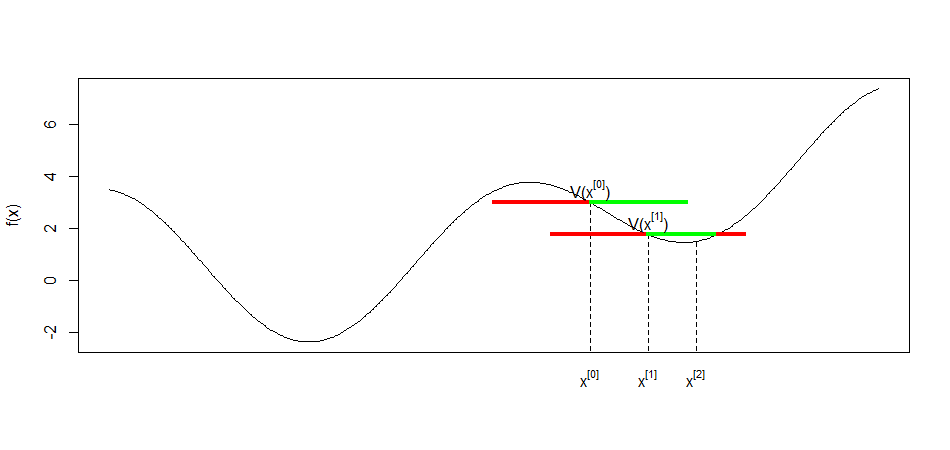
\includegraphics[width=0.75\textwidth]{figure_man/local-search.png}
\end{center}
\vspace{-0.5cm}
%\begin{figure}
%<<echo=FALSE, fig.height=4.25>>=
%int = seq(0,4, length.out = 500)
%f = function(x) x^1.1 * sin(x-2) + 1 - 2.5*sin(3*x-1.5)
%plot(int, f(int), type="l", xlab = "", ylab = "f(x)", xaxt="n")
%x = 2.5
%rad = 0.5
%lines(c(x, x), c(-3, f(x)), lty = 2)
%area = seq(x - rad, x+rad, length.out=200)
%col_vec = c("red", "green")
%points(area, rep(f(x), 200), col = col_vec[(f(area)<f(x))+1], pch=15, cex=0.5)

%x = 2.8
%rad = 0.5
%lines(c(x, x), c(-3, f(x)), lty = 2)
%area = seq(x - rad, x+rad, length.out=200)
%col_vec = c("red", "green")
%points(area, rep(f(x), 200), col = col_vec[(f(area)<f(x))+1], pch=15, cex=0.5)


%lines(c(3.05,3.05), c(-3, f(3.05)), lty=2)
%axis(1, c(2.5, 2.8, 3.05), labels = c(expression(x[0]), expression(x[1]), expression(x[2])),tick=F)
%@
%\caption{local search; green: acceptance range, red: rejection range}
%\end{figure}
\footnotesize{Stochastic local search; green: acceptance range, red: rejection range}
\end{vbframe}

\begin{vbframe}{Metropolis algorithm}
\begin{itemize}
\item Stochastic local search strongly depends on the initialization of $x^{[0]}$ and the neighborhood.
\item Danger of ending up in local minima.
\item Sensible: temporarily allow worse candidate combinations.
\item Metropolis: accept candidate solutions from previous rejection range ($\Delta f > 0$) with probability $\P(\text{acceptance} | \Delta f) = exp(-\frac{\Delta f}{T}).$
\item $T$ denotes the \textbf{temperature}
\end{itemize}

\vspace{-0.5cm}
\begin{center}
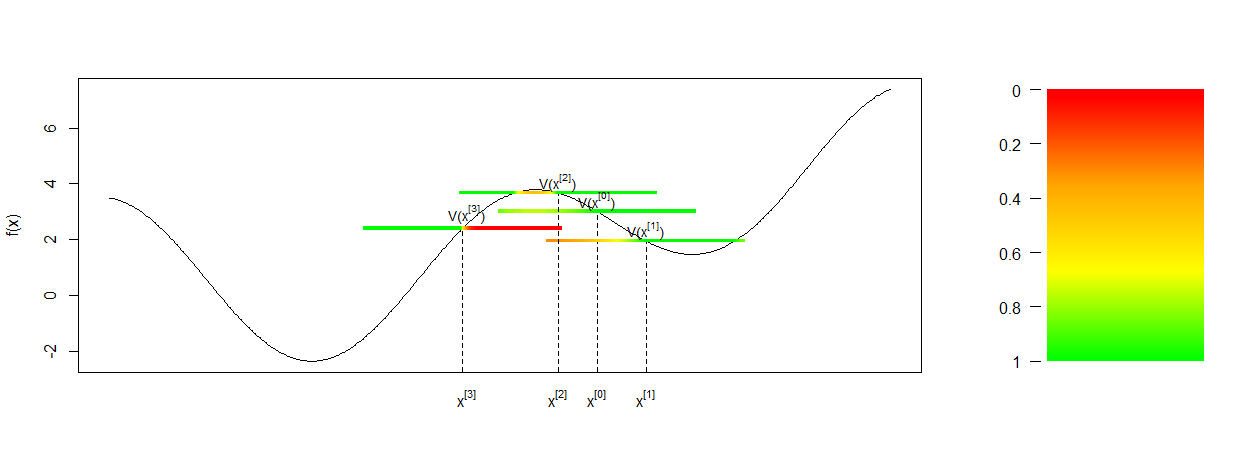
\includegraphics[width=0.85\textwidth]{figure_man/metropolis-algorithm.png}
\end{center}
\vspace{-0.6cm}

%\begin{figure}
%<<echo=FALSE, fig.height=4.25>>=
%PDelta = function(Delta_f, Temp) {
%  ret = exp(- Delta_f / (Temp))
%  ret[ret>1] = 1
%  ret
%}


%layout(matrix(1:2, nrow = 1), width = c(5,1.5), height = rep(1,2))


%int = seq(0,4, length.out = 500)
%f = function(x) x^1.1 * sin(x-2) + 1 - 2.5*sin(3*x-1.5)
%plot(int, f(int), type="l", xlab = "", ylab = "f(x)", xaxt="n")
%x = 2.5
%rad = 0.5
%lines(c(x, x), c(-3, f(x)), lty = 2)
%area = seq(x - rad, x+rad, length.out=200)
%col_vec = c("yellow", "green")

%rbPal <- colorRampPalette(c('red','orange', "yellow", "green"))
%col_smooth <- rbPal(50)[as.numeric(cut(seq(0,1,0.02),breaks = 50))]

%points(area, rep(f(x), 200),
%       col = col_smooth[findInterval(PDelta(f(area)-f(x), Temp=3), seq(0,1,0.02))],
%       pch=15, cex=0.5)

%x = 2.75
%rad = 0.5
%lines(c(x, x), c(-3, f(x)), lty = 2)
%area = seq(x - rad, x+rad, length.out=200)
%col_vec = c("orange", "green")
%points(area, rep(f(x), 200),
%       col = col_smooth[findInterval(PDelta(f(area)-f(x), Temp=1.5), seq(0,1,0.02))],
%       pch=15, cex=0.5)
%x = 2.3
%rad = 0.5
%lines(c(x, x), c(-3, f(x)), lty = 2)
%area = seq(x - rad, x+rad, length.out=200)
%points(area, rep(f(x), 200),
%       col = col_smooth[findInterval(PDelta(f(area)-f(x), Temp=0.15), seq(0,1,0.02))],
%       pch=15, cex=0.5)

%x = 1.81
%rad = 0.5
%lines(c(x, x), c(-3, f(x)), lty = 2)
%area = seq(x - rad, x+rad, length.out=200)
%points(area, rep(f(x), 200),
%       col = col_smooth[findInterval(PDelta(f(area)-f(x), Temp=0.15), seq(0,1,0.02))],
%       pch=15, cex=0.5)

%axis(1, c(2.5, 2.75, 2.3, 1.83), labels = c(expression(x[0]), expression(x[1]), expression(x[2]) , expression(x[3])),tick=F)

%#legend
%legend_image <- as.raster(matrix(col_smooth, ncol=1))
%plot(c(0,1),c(0,1), type = 'n', axes = F, xlab = '', ylab = '', main = "")
%rasterImage(legend_image, 0, 0, 1, 1)
%axis(2, at = seq(0, 1, l = 6), labels = seq(1, 0, l = 6), tick = T, las=1,
%     lwd = 0, lwd.ticks = 1)
%@
%\caption{Simulated Annealing schematic, colors: P(acceptance)}
%\end{figure}
\footnotesize{Simulated annealing schematic, colors: $\P$(acceptance)}

\framebreak

\begin{small}
\begin{itemize}
\item New parameter $T$ describes temperature/progress of the system.
\item The higher $T$, the higher the probability to accept worse $\bm{x}$.
\item Atomical view: individual atoms (solution points) of the system can move more freely
\item Local minima can be escaped again, but no convergence can be achieved at constant temperature
\item We come across an important principle of optimization:\\
  \textbf{exploration (high T) vs. exploitation (low T)}
\end{itemize}
\end{small}
\vspace{-0.3cm}
\begin{center}
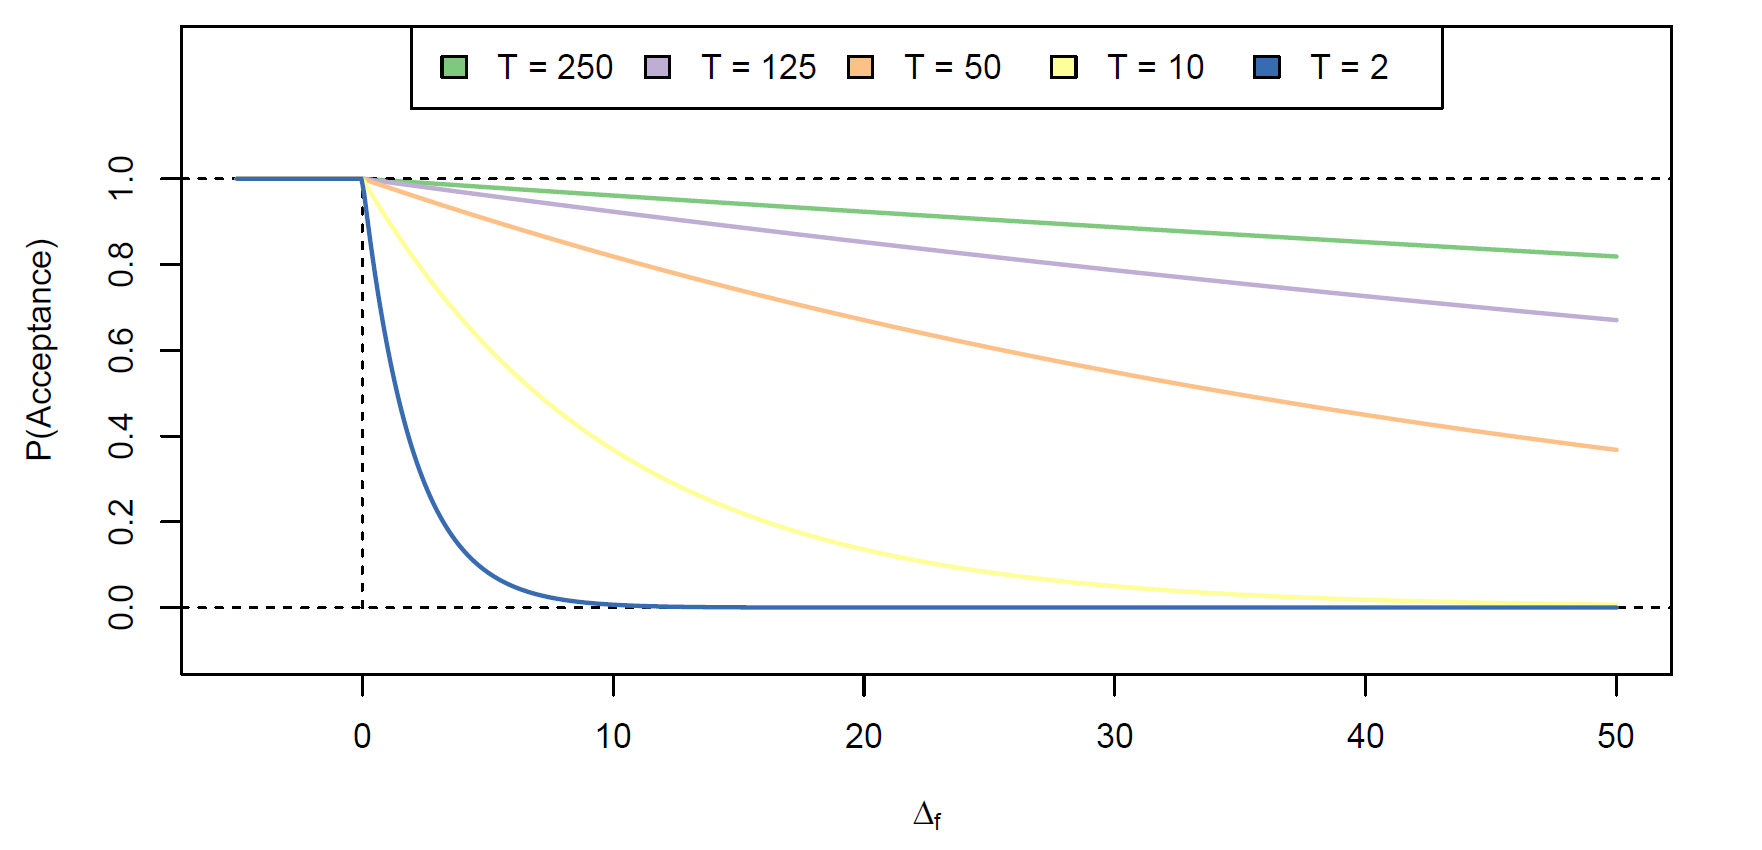
\includegraphics[width=0.6\textwidth]{figure_man/metropolis-algorithm2.png}
\end{center}


%\begin{figure}
%<<echo=FALSE>>=
%library("RColorBrewer")
%Delta = seq(-5, 50, length.out= 500)

%colvec = brewer.pal(5, "Accent")
%plot(Delta, PDelta(Delta, 250), type = "l", ylim = c(-0.1,1.3), xlab = expression(Delta[f]), ylab = "P(Acceptance)", col = colvec[1], lwd = 2, yaxt="n")
%axis(2, seq(0,1, by=.2))
%abline(h=c(0,1), lty = 2)
%lines(c(0,0), c(0,1), lty=2)
%points(Delta, PDelta(Delta, 125), type = "l", col = colvec[2], lwd = 2)
%points(Delta, PDelta(Delta, 50), type = "l", lwd = 2, col = colvec[3])
%points(Delta, PDelta(Delta, 10), type = "l", lwd = 2,col = colvec[4])
%points(Delta, PDelta(Delta, 2), type = "l", lwd = 2, col = colvec[5])
%legend("top", paste("T =", c(250,125,50,10,2)), fill=colvec, ncol=5)
%@
%\caption{Representation of acceptance probability}
%\end{figure}
%Representation of acceptance probability

\end{vbframe}

\begin{vbframe}{Simulated Annealing}
\begin{itemize}
\item Approach now: start with high temperature to search the whole system (\textbf{exploration})
\item Slowly lower temperature to reach a minimum \\
$\Rightarrow$ sequence of temperatures $T^{[t]}, t \in \N$
\item If temperature depends on simulation time, the procedure is called \textbf{simulated annealing}.
\item Temperature is often kept constant several iterations at a time to search the space of candidate solutions, then multiplied by coefficient $0<c<1$:

$$
T^{[t+1]} = c \cdot T^{[t]}
$$
\end{itemize}

\framebreak


\framebreak
(Choice of) optimization parameters \\
\begin{itemize}
\item Temperature $T$: for any optimization problem, the initial temperature can be the average of a number of random function values.
\vspace{0.1cm}
\item Temperature coefficient $c$: typically between 0.6 and 0.9 ($c<1$)
\vspace{0.1cm}
\item Iterations at the same temperature: typically between 50-100
\vspace{0.1cm}
\item Range $\gamma$: defines area around $\bm{x}^{[t]}$ in which next candidate solution set $\bm{x}^{[t+1]}$ is searched (depends strongly on objective function)
\end{itemize}

\end{vbframe}

% \begin{vbframe}{Simulated Annealing: Algorithmus}
% \begin{algorithm}[H]
%   \begin{footnotesize}
%   \begin{center}
%   \caption{Simulated Annealing}
%    \begin{algorithmic}[1]
%     \State Generiere zufällige Startlösung $x$
%     \State Setze $x_{best} = x$
%     \State Wähle eine monoton fallende Folge von positiven Temperaturwerten $(T_{k})_{k \in N}$
%     \State Wähle Minimale Tmperatur $T_{min}$ als Abbruchkriterium
%     \State Setze $k = 1$
%        \While{$T_{k} >  T_{min}$}
%         \State Wähle in Umgebung von x einen zufälligen Punkt $x_{new}$ aus
%         \If{$f(x_{new}) < f(x)$}  {setze $x = x_{new}$}
%         \ElsIf{
%         {{setze $x = x_{new}$ mit Wahrscheinlichkeit $exp(- \frac{f(x_{new})-f(x)}{T_k})$}}}
%         \EndIf
%         \If{$f(x) < f(x_{best})$} {update $x_{best} = x$}
%         \EndIf
%         \State $k = k + 1$
%       \EndWhile
%     \end{algorithmic}
%     \end{center}
%     \end{footnotesize}
% \end{algorithm}
% \end{vbframe}

\begin{frame}
\frametitle{Example: simulated annealing}


  \begin{center}
  \only<1>{
  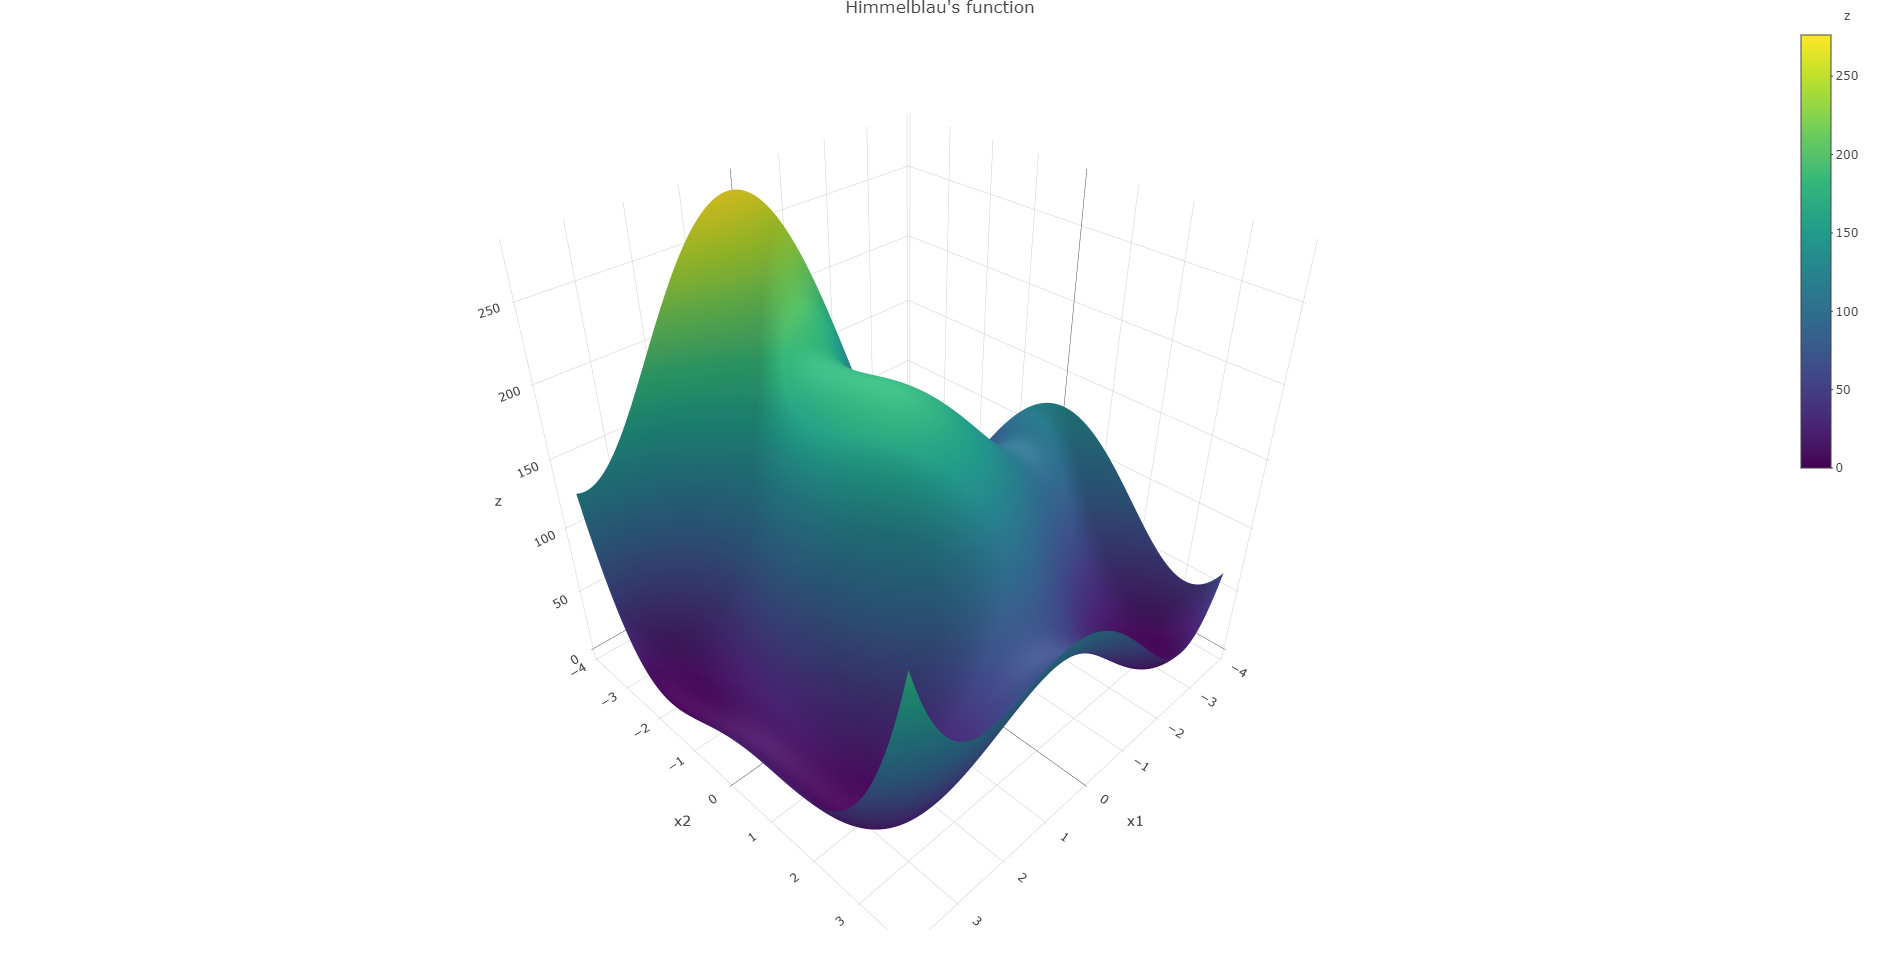
\includegraphics[width=0.54\textwidth]{figure_man/sa-himmelblauFun3D.png}
  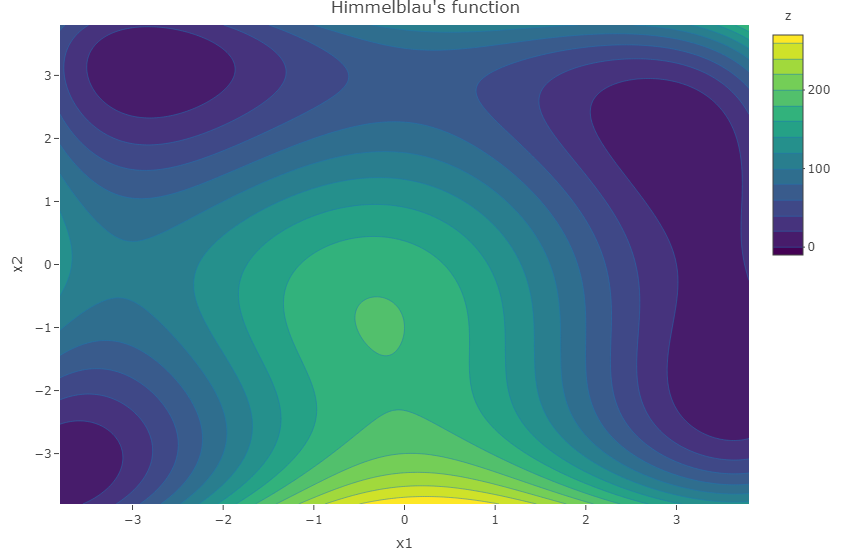
\includegraphics[width=0.44\textwidth]{figure_man/sa-himmelblauFun2D.png}\\

          \begin{itemize}
            \item Himmelblau's function has several local optima.
            \item We perform $100$ iterations of simulated annealing with the following settings: 
            \begin{itemize}
            \item Proposal points are sampled from a normal distribution ($\sigma = 1.5$) around the current point
            \item Initial temperature of $T^{[0]} = 200$
            \item Constant temperature for the first $50$ iterations
            \item Afterwards, temperature drops by a multiplicative factor of $c = 0.8$ in every iteration
          \end{itemize}
          \end{itemize}}%

  \only<2>{

    \begin{figure}
      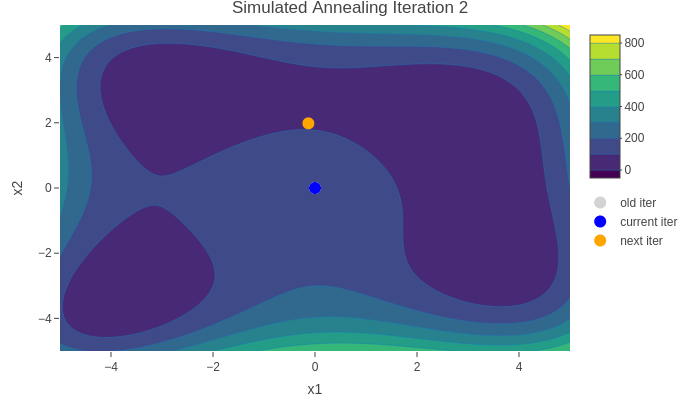
\includegraphics[width=0.45\textwidth]{figure_man/sa-iter2.png}    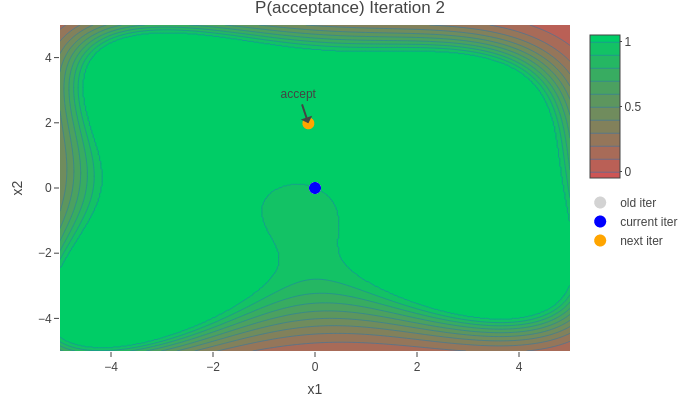
\includegraphics[width=0.45\textwidth]{figure_man/sa-probs-iter2.png} \\
    \end{figure}
          \begin{tiny}
      Left: Optimization surface of the Himmelblau function. Right: Acceptance probability $\P(\text{acceptance})$. 
      \end{tiny} 

    \begin{itemize}
          \item The orange dot is the starting point $(0, 0)$ \\ of the optimization.
          \item For the first $50$ iterations, the temperature is set to $T = 200$. 
          \item In the beginning, almost every point is accepted
    \end{itemize}}%

  \only<3>{

    \begin{figure}
      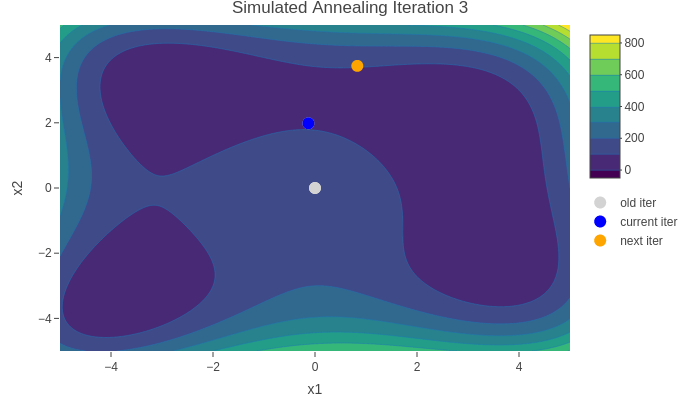
\includegraphics[width=0.45\textwidth]{figure_man/sa-iter3.png}    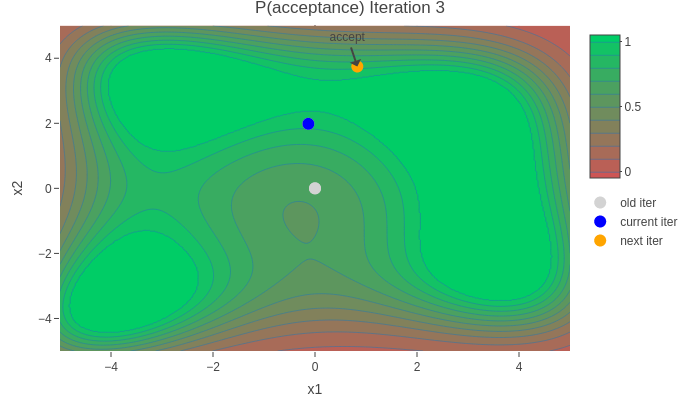
\includegraphics[width=0.45\textwidth]{figure_man/sa-probs-iter3.png} \\
    \end{figure}
          \begin{tiny}
      Left: Optimization surface of the Himmelblau function. Right: Acceptance probability $\P(\text{acceptance})$. 
      \end{tiny} 

    \begin{itemize}
          \item The orange dot is the starting point $(0, 0)$ \\ of the optimization.
          \item For the first $50$ iterations, the temperature is set to $T = 200$. 
          \item In the beginning, almost every point is accepted
    \end{itemize}}%

  \only<4>{

    \begin{figure}
      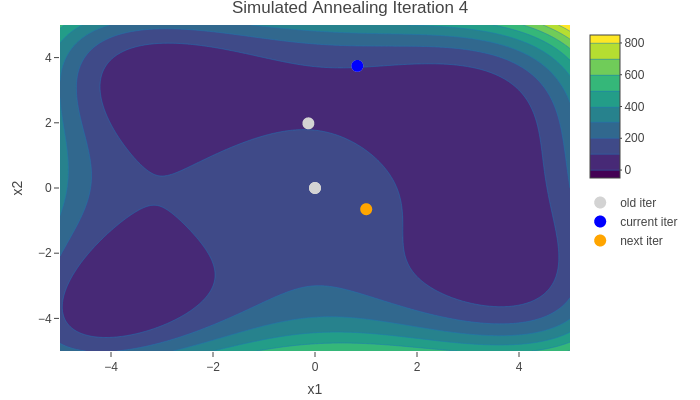
\includegraphics[width=0.45\textwidth]{figure_man/sa-iter4.png}    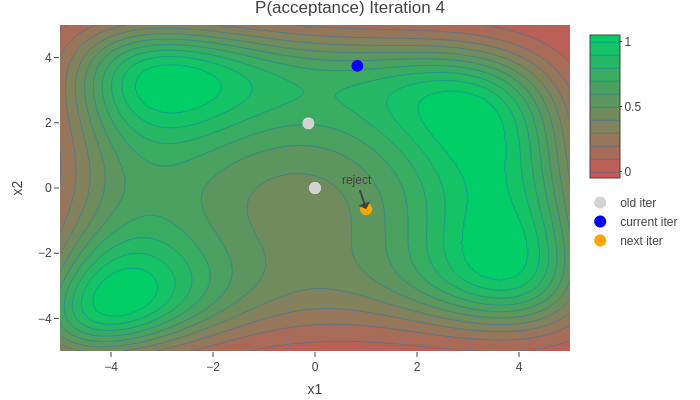
\includegraphics[width=0.45\textwidth]{figure_man/sa-probs-iter4.png} \\
    \end{figure}
          \begin{tiny}
      Left: Optimization surface of the Himmelblau function. Right: Acceptance probability $\P(\text{acceptance})$. 
      \end{tiny} 

    \begin{itemize}
          \item The orange dot is the starting point $(0, 0)$ \\ of the optimization.
          \item For the first $50$ iterations, the temperature is set to $T = 200$. 
          \item In the beginning, almost every point is accepted
          \item Sometimes we end up with a point that is rejected (e.g., iteration 4) 
    \end{itemize}}%

  \only<5>{

    \begin{figure}
      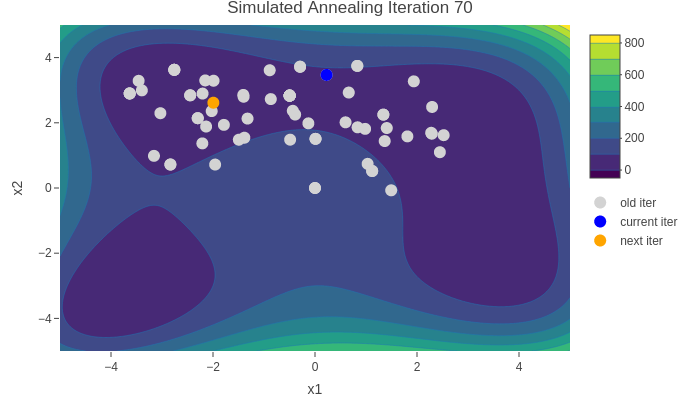
\includegraphics[width=0.45\textwidth]{figure_man/sa-iter70.png}    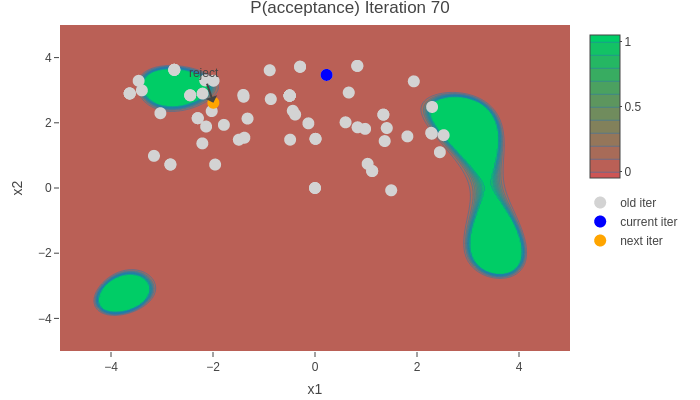
\includegraphics[width=0.45\textwidth]{figure_man/sa-probs-iter70.png} \\
    \end{figure}
          \begin{tiny}
      Left: Optimization surface of the Himmelblau function. Right: Acceptance probability $\P(\text{acceptance})$. 
      \end{tiny} 

    \begin{itemize}
          \item From iteration $50$ on, temperature starts $T$ to drop by the multiplicative factor of $c = 0.8$ in every iteration
          \item We see that we cannot move as freely anymore. 
    \end{itemize}}%

  % \only<3>{
  %   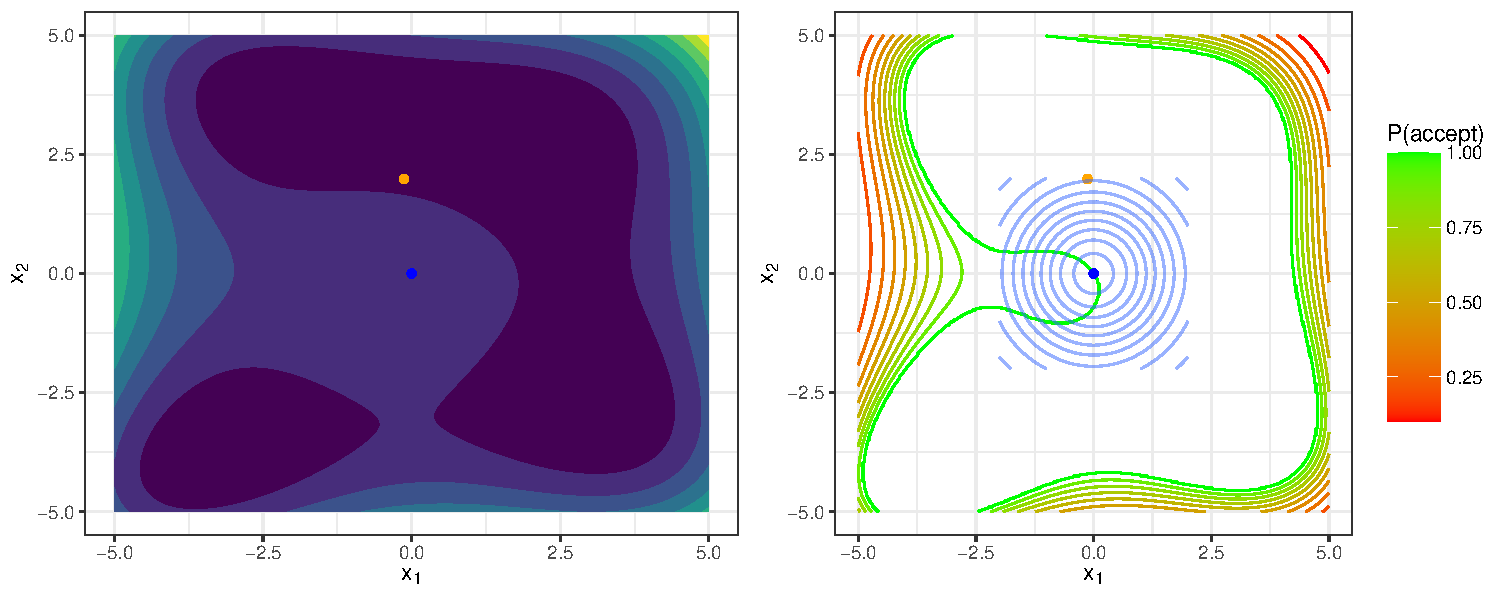
\includegraphics[width=0.49\textwidth]{figure_man/sa-iter1.png}
  %   \includegraphics[width=0.49\textwidth]{figure_man/sa-probs-iter1.png}\\

  %   \begin{itemize}
  %         \item Left: The point $\xv^{[2]} = (x,y)$ was sampled in iteration 2, and accepted. 
  %         \item Right: Acceptance probability $P = \exp(-\frac{\Delta f}{T})$ for $\xv^{[2]} = (x,y)$ is $m$. 
  %   \end{itemize}}%

  % \only<4>{
  %   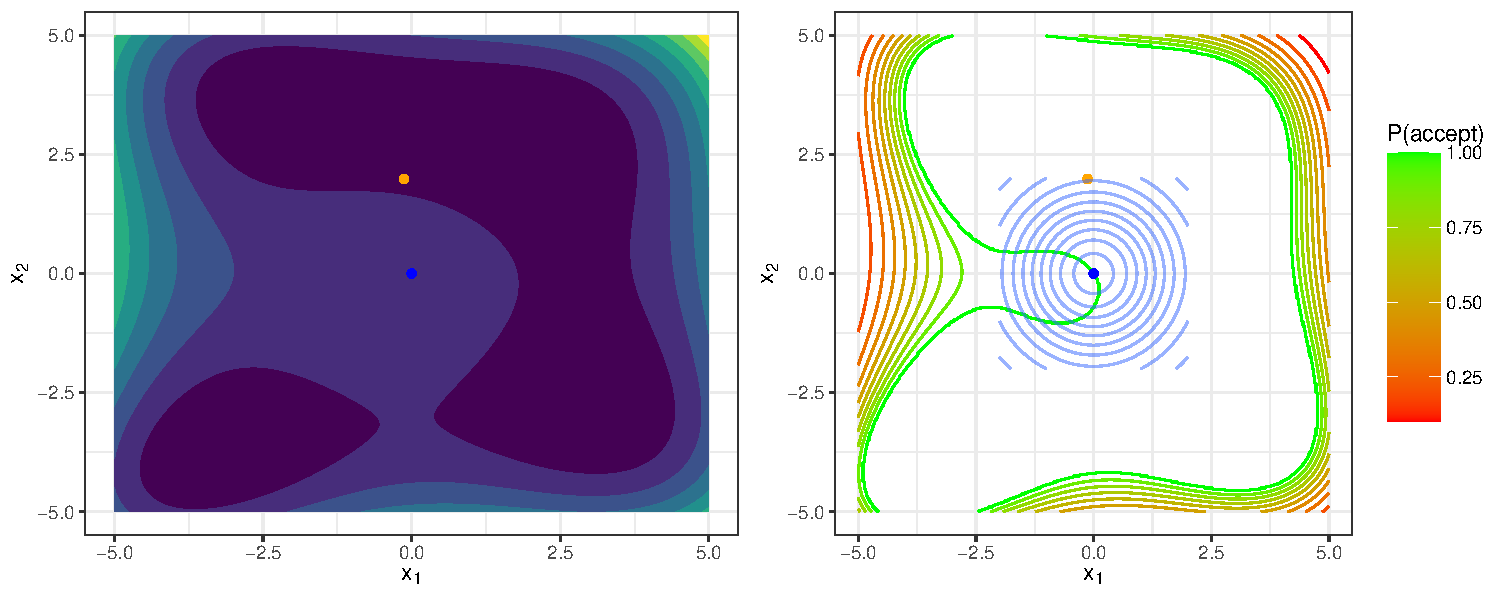
\includegraphics[width=0.49\textwidth]{figure_man/sa-iter1.png}
  %   \includegraphics[width=0.49\textwidth]{figure_man/sa-probs-iter1.png}\\

  %   \begin{itemize}
  %         \item Left: We repeat the procedure for $50$ iterations without changing the temperature.  
  %   \end{itemize}}%

  % \only<4>{
  %   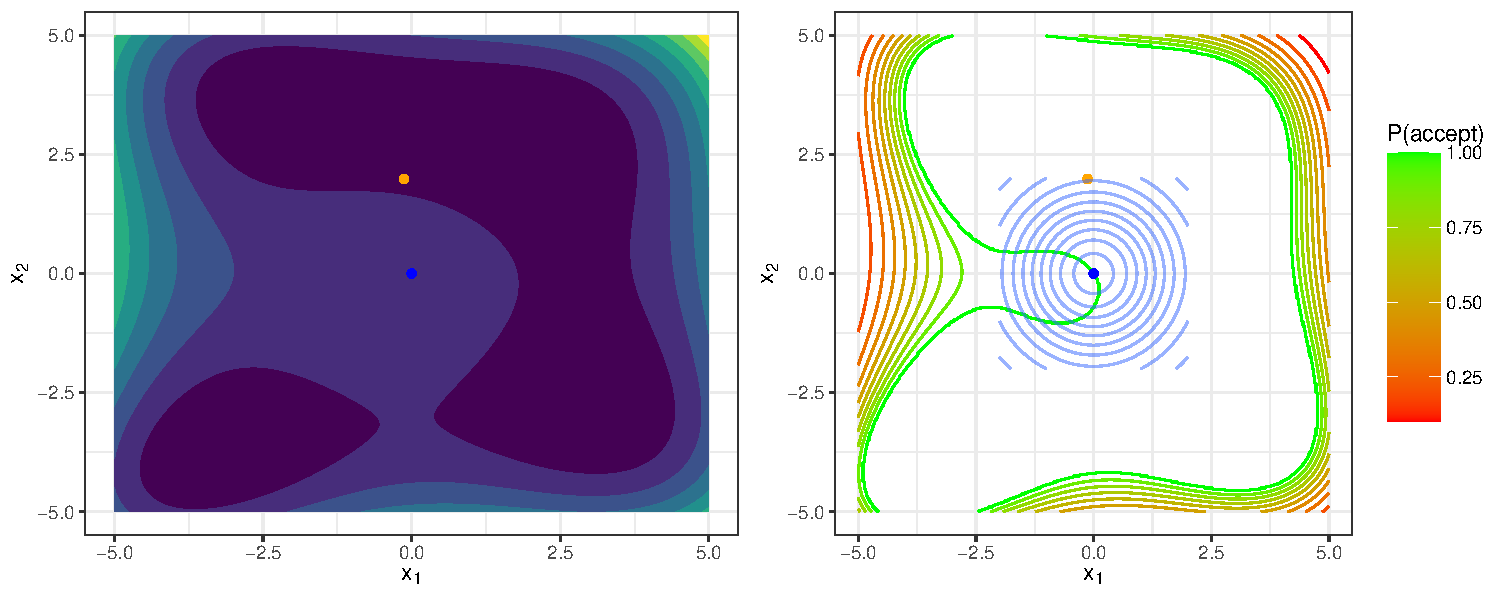
\includegraphics[width=0.49\textwidth]{figure_man/sa-iter1.png}
  %   \includegraphics[width=0.49\textwidth]{figure_man/sa-probs-iter1.png}\\

  %   \begin{itemize}
  %         \item The next 50 iterations are performed with a temperature of $T = 160$. We see that the sampled points focus more around the (local) optima of the function
  %   \end{itemize}}%

  % \only<4>{
  %   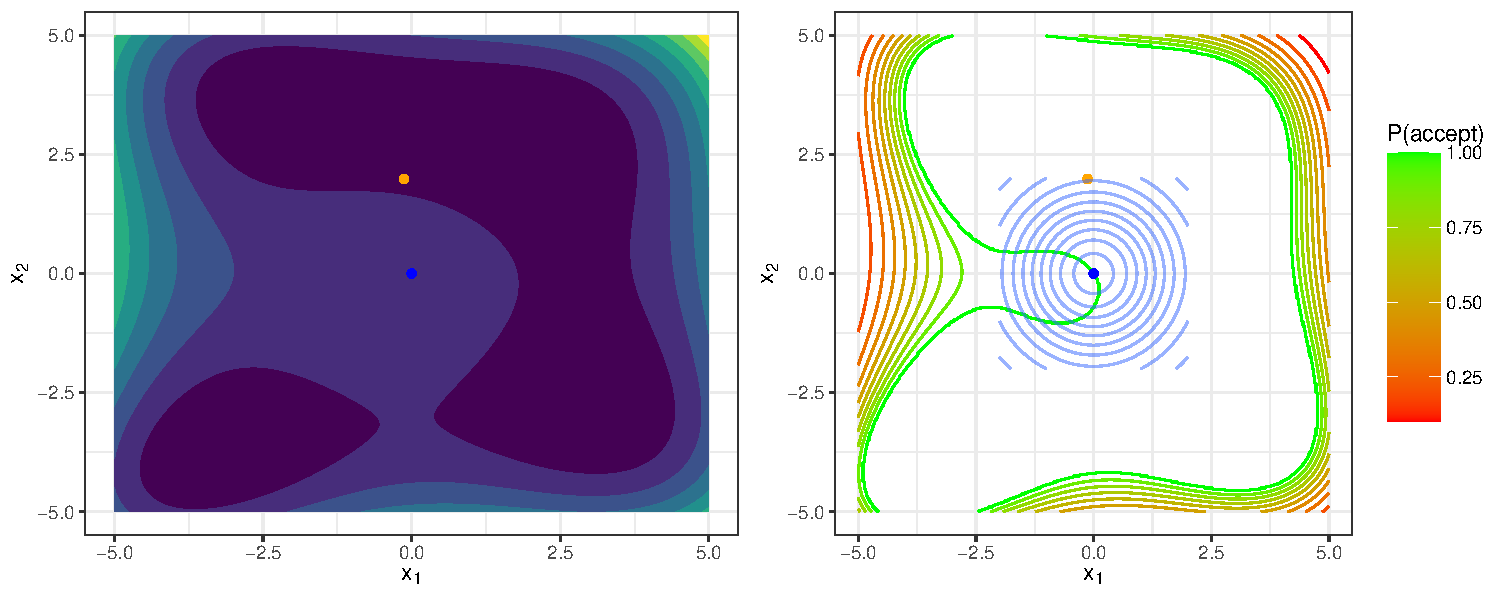
\includegraphics[width=0.49\textwidth]{figure_man/sa-iter1.png}
  %   \includegraphics[width=0.49\textwidth]{figure_man/sa-probs-iter1.png}\\

  %   \begin{itemize}
  %         \item After 100 iterations, the temperature would change again. But we stop here. 
  %   \end{itemize}}%


  % %\only<3>{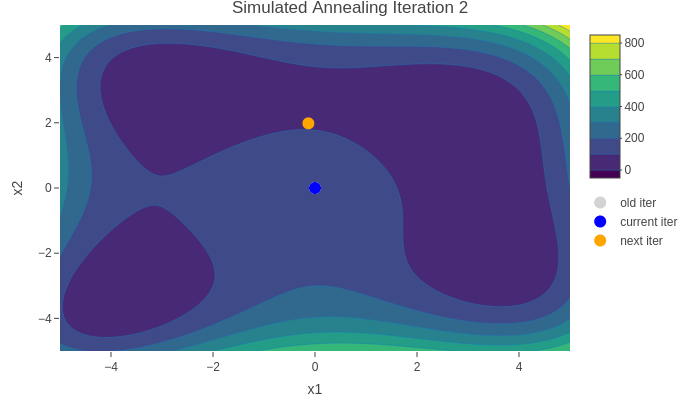
\includegraphics[height = 5cm, width=5.5cm]{figure_man/sa-iter2.png}}%
  % %\only<3>{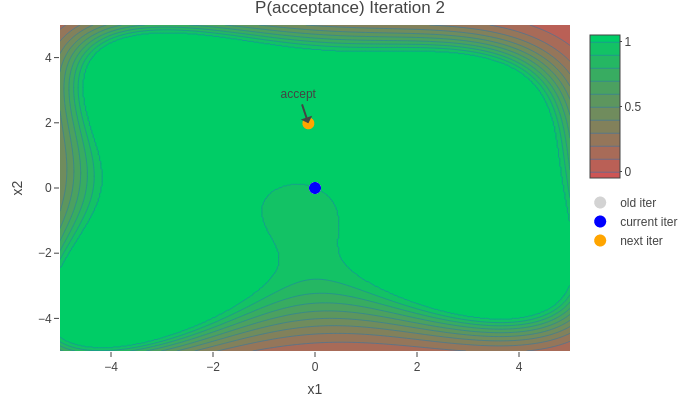
\includegraphics[height = 5cm, width=5.5cm]{figure_man/sa-probs-iter2.png}%
  %  % \begin{itemize}
  %   %      \item Left: new point
  %    %     \item Right: probability of acceptance $P = \exp(-\frac{\Delta f}{T})$ regarding the new point
  %   %\end{itemize}}%

  % \only<3>{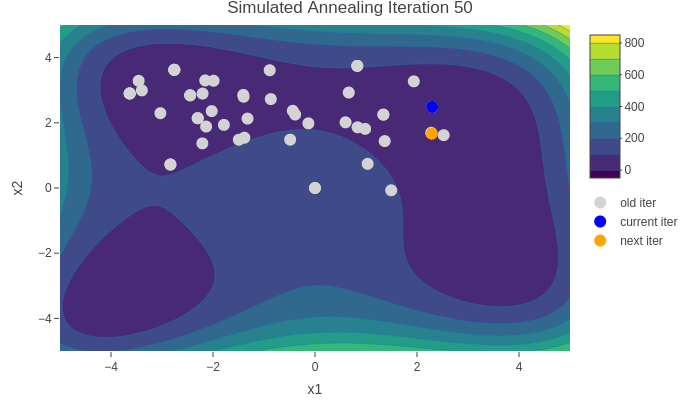
\includegraphics[width=0.49\textwidth]{figure_man/sa-iter50.png}
  %           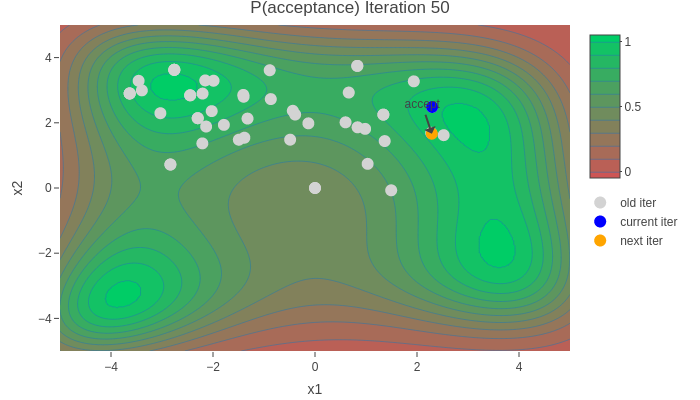
\includegraphics[width=0.49\textwidth]{figure_man/sa-probs-iter50.png}\\

  %           \begin{itemize}
  %           \item Left: temperature at the beginning constantly high; points scatter strongly (exploration)
  %           \item Right: Downgrading of the acceptance probability still clearly visible (contour lines can still be clearly differentiated)
  %           \end{itemize}}%
  % \only<4>{\includegraphics[width=0.49\textwidth]{figure_man/sa-iter100.png}
  %           \includegraphics[width=0.49\textwidth]{figure_man/sa-probs-iter100.png}\\

  %           \begin{itemize}
  %           \item Left: temperature has already decreased significantly, points scatter less, \enquote{solidification} begins (exploitation)
  %           \item Right: Downgrading of the acceptance probability hardly perceptible any more (contour lines can hardly be differentiated anymore)
  %           \end{itemize}}%

  \end{center}
  \end{frame}



\endlecture
\end{document}

